\documentclass[12pt, twoside]{article}
\usepackage[utf8]{inputenc}
\usepackage[english]{babel}

\usepackage{amsthm}
\usepackage{a4wide}
\usepackage{graphicx}
\usepackage{caption}
\usepackage{amssymb}
\usepackage{amsmath}
\usepackage{mathrsfs}
\usepackage{euscript}
\usepackage{graphicx}
\usepackage{subfig}
\usepackage{caption}
\usepackage{color}
\usepackage{bm}
\usepackage{tabularx}
\usepackage{adjustbox}


\usepackage[toc,page]{appendix}

\usepackage{comment}
\usepackage{rotating}

\DeclareMathOperator*{\argmax}{arg\,max}
\DeclareMathOperator*{\argmin}{arg\,min}

\renewcommand{\baselinestretch}{1.5}


\numberwithin{equation}{section}

\newcommand*{\No}{No.}
\begin{document}

\title{\bf Quasi-periodic time series clustering for human activity recognition\thanks{This research was supported by RFBR, project ..., and by Government of the Russian Federation, agreement ...}}
\date{}
\author{}
\maketitle

\begin{center}
\bf
A.\,V.~Grabovoy\footnote{Moscow Institute of Physics and Technology, grabovoy.av@phystech.edu}, V.\,V.~Strijov\footnote{Moscow Institute of Physics and Technology, strijov@ccas.ru}

\end{center}

{\centering\begin{quote}
\textbf{Annotation:} This paper analyses the periodic signals in the time series to recognize human activity by using a mobile accelerometer. 
Each point in the timeline corresponds to a segment of historical time series. This segments form a phase trajectory in phase space of human activity.
The principal components of segments of the phase trajectory are treated as feature descriptions at the point in the timeline.
The paper introduces a new distance function between the points in new feature space.
To reval changes of types of the human activity the paper proposes an algorithm. This algorithm clusters points of the timeline by using a pairwise distances matrix.
The algorithm was tested on synthetic and real data. This real data were obtained from a mobile accelerometer.


\smallskip
\textbf{Key words}: time series; clustering; segmentation; recognition of physical activity; principal component method.

\smallskip
%\textbf{DOI}: 00.00000/00000000000000
\end{quote}
}

\section{Introduction}
Analysis of the human physical activity is carried out by using mobile phones, smart watches and another wearable devices~\cite{kwapisz2010, wang2014}.
These devices uses an accelerometer, gyroscope and magnetometer. 
The main purpose of this work is construct an informative low-dimensional representation to generate features of a human behaviour~\cite{Ignatov2015, Olivares2012}. This representation also defines the phase of the movements~\cite{motrenko2015, cinar2018}.
Examples of the physical action segment are a step, a step of running, a single squat, a single jump, etc.
This work considers a sequence that consists of at least two consecutive segments that correspond to the same type of human activity.

\begin{figure}[h!t]\center
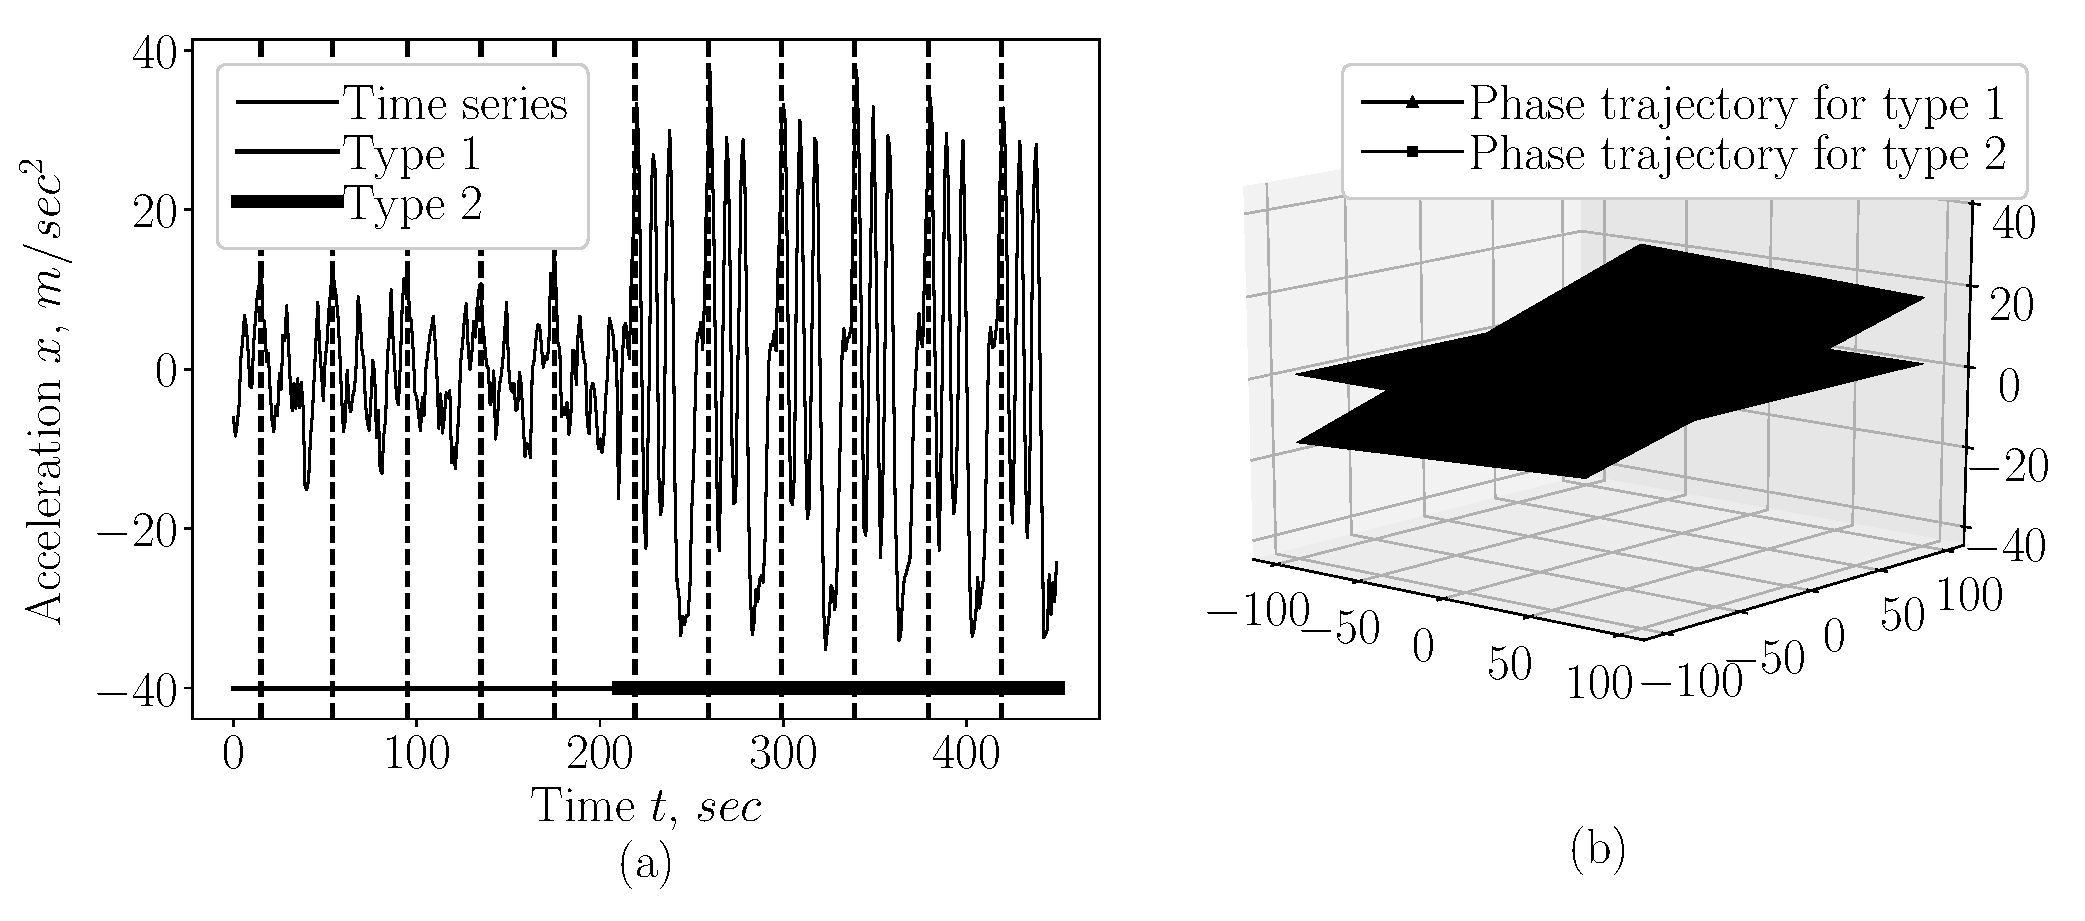
\includegraphics[width=1\textwidth]{results_eng/introduction}
\caption{A time series with clustering:  a) time series with assessor markings on clusters and markings at beginning of each quasi-periodic segment; b) projection of phase trajectories on the two principal components}
\label{fig:introduction:1}
\end{figure}

Time series are objects of complex structure. 
The method of constructing feature vectors for points is very important for their clustering.
In this work, the object of analysis is a point on the time axis.
Any sample set is collected as samples, taken before this point.
This work investigates the clustering problem: all points on the time line are labeled with a label from some finite set of labels.
Each label corresponds to physical action.
A \textit{segment} of time series corresponds to physical action. For example: a step with two legs when walking, or a step with two legs when running.
A sequence of segments that forms a quasi-periodic sequence is called the \textit{chain}.
A sequence of points $\{b_t\}_{t=1}^{N}$ is called \textit{quasi-periodic} with period of $T$, if for all $t$ there is a $\Delta$, such that:
\begin{equation}
\label{eq:int:1}
\begin{aligned}
b_t \approx b_{t+T+\Delta}, \quad \left|\Delta\right| \ll T.
\end{aligned}
\end{equation}
An example of clustering and splitting a series into segments is shown in fig.~\ref{fig:introduction:1}.a. 
Fig.~\ref{fig:introduction:1}.a shows an example of time series clustering and segmentation.
The time series is splitted into two characteristic type of segments: Type~1 and Type~2. 
This time series contains two quasi-periodic chains of actions.

The proposed solution of the clustering problem consists of two stages.
First, an algorithm for local approximation of time series by using the principal component method~\cite{Shiglavsi1997} obtains a feature description of points in the time series.
\textit{Local information} of the time series means that only a certain neighborhood of a point is used to describe the features of their points.
A few main components of the phase trajectory segment are considered as a feature description of a time series point.
Fig.~\ref{fig:introduction:1}.b shows the two first principal components of a phase trajectorie, and the projection of the phase trajectory to these components.
Two trajectories relate to different physical actions: Type~1 and Type~2, in the time series.
The planes that are generated by these principal components are different.
It separates Type~1 and Type~2 as two different actions.
%переписать
Second the distance function between points in the new feature space.
This function is the distance between two bases of some subspaces within the phase space of a time series.
It can be explained by using fig~\ref{fig:introduction:1}.b. The function is considered between two planes, which are defined by two different bases for the Type1 and Type2 segments.
Points clustered by using a pairwise distance matrix.
The segmentation problem is solved by using the main components~\cite{motrenko2015} of the phase trajectory in each cluster separately.

The method assumes that periods of different segments vary slightly. Minimum and maximum periods of segments are given. The number of different segments in the time series is known too.
It is also assumed that the type of segments in time does not change often. For example, a human runs for 10 seconds and then walks for 15 seconds and so on.

The analysis of the proposed clustering method is carried out on synthetic and real data. 
The experiment on the segmentation of the time series was carried out on simple sinusoidal signals with random amplitude and frequency.
Synthetic dataset constructed by using the sum of the first few terms of the Fourier series with random coefficients. 
Real data was received by using a mobile accelerometer, which took readings during exercise of a person. All time series consist of two or three type of action such as walking, running, squats.

\section{Related work}
The paper~\cite{kwapisz2010} describes a method for constructing a feature description based on expertly defined generating functions.
The paper~\cite{lukashin2003} proposes a method for constructing features based on the data generation hypothesis.
A combined feature description is introduced in the paper~\cite{Ivkin2015} based on these methods.
The paper~\cite{Katrutsa2015} consider the problem of construction a feature space. The article proposes a criterion for the redundancy of the selected features.

The paper~\cite{Ignatov2015} is the closest one to our research.
It proposes a method for human physical activity recognition.
To extract the fundamental period they construct the phase trajectory matrix, applying a technique of the principal component analysis. 
This method allows you to find and classify segments in time series with great accuracy. But this method can work only with time series, in which all segments belong to the same characteristic action.

The paper~\cite{motrenko2015} is one of the closest to our research.
It searches for the beginning of a segment within a quasiperiodic signal, which consists of only one chain of actions.
Their method is based on the study of the phase space, namely, the search for a stable hyperplane that divides the phase space into two equal parts.
The points that are close to this hyperplane are selected as the beginning and ending of the segment.
The article~\cite{motrenko2015} proposes to project the phase space into two principal components. The beginning of each segment should be highlighted.
This method finds the beginning of a segment in the case when the time series consists of one type of signal.

The paper~\cite{cinar2018} is also close to our research. 
The article proposes a method for searching for a periodic structure in a series by using the LSTM model with attention mechanism.
This method has the same disadvantage as the previous method~\cite{motrenko2015}. This method finds the beginning of a segment in the case when the time series consists of one type of signal.


\section{Time series clustering problem}

There given a time series
\begin{equation}
\label{eq:st:1}
\begin{aligned}
\textbf{x} \in \mathbb{R}^{N},
\end{aligned}
\end{equation}
where~$N$ is a number of samples in the time series. The time series consists of a sequence of segments,
\begin{equation}
\label{eq:st:2}
\begin{aligned}
\textbf{x} = [\textbf{v}_1, \textbf{v}_2, \cdots, \textbf{v}_M],
\end{aligned}
\end{equation}
where~$\textbf{v}_i$ is a segment from the set of segments~$\mathbf{V}$. 
It is supposed that the time series $\textbf{x}$ contains some $\textbf{v}_i$ from $\textbf{V}$.
%which are observed in the time series $\textbf{x}$. 
For all~$i$ either~$[\textbf{v}_{i-1},\textbf{v}_{i}]$ or~$[\textbf{v}_{i},\textbf{v}_{i+1}]$  is a  chain of actions. Fig.~\ref{fig:statement:1}.a shows an example of segments $\textbf{v}_i$.
Each segments $\textbf{v}_{i}$ has no more than $T$ elements, $\left|\textbf{v}_{i}\right| \leq T$. 
The set $V$ has $K$ different types of segments, $\left|\mathbf{V}\right| = K$. 
Fig.~\ref{fig:statement:1}.a shows an example of segments, which are constructed the chain of action~$[\textbf{v}_{i-1}, \textbf{v}_{i}, \textbf{v}_{i+1}]$.
%The figure shows an example of $ 1 $, $ 2 $ segments that belong to segments of the same type.

%Let the set of segments~$\mathbf{V}$ satisfies the following properties:

%\begin{equation}
%\label{eq:st:3}
%\begin{aligned}
%\left|\mathbf{V}\right| = K, \quad \textbf{v} \in \mathbf{V}~\left|\textbf{v}\right| \leq T,
%\end{aligned}
%\end{equation}
%where~$\left|\mathbf{V}\right|$ is a number of different action in the set of segments $\mathbf{V},$~$\left|\textbf{v}\right|$ is a length of segment,~$K$ is a number of different action in the time series $\textbf{x}$ and~$T$ is a length of maximum segment.

\begin{figure}[h!t]\center
\includegraphics[width=1\textwidth]{results_eng/statement}
\caption{A time series and example of local information of points:  a) time series example of local information of time point~$t = 90$; b) projection of phase trajectories on the two principal components and example of segment~$\textbf{s}_t$ in time point~$t = 90$}
\label{fig:statement:1}
\end{figure}

Construct the mapping of points into classes for their clustering
\begin{equation}
\label{eq:st:4}
\begin{aligned}
a : t \to \mathbb{Y} = \{1,\cdots, K\}, 
\end{aligned}
\end{equation}
where~$t \in \{1,\cdots, N\}$ is a point in the timeline which defines the time series $\textbf{x}$.
Let the map~$a$ satisfy the following properties:
\begin{equation}
\label{eq:st:5}
\begin{aligned}
\begin{cases}
    a\left(t_1\right) = a\left(t_2\right), &  \text{if time moments } t_1, t_2 \text{ relate to similar type of segments,}\\
    a\left(t_1\right) \not= a\left(t_2\right), &  \text{if time moments } t_1, t_2 \text{ relate to different type of segments.}
\end{cases}
\end{aligned}
\end{equation}

Each point~$t$ corresponds to a label~$y_t$ from the set $\mathbb{Y} =  \{1,\cdots,K\}$:
%Consider following markup of the time series points:
\begin{equation}
\label{eq:st:6}
\begin{aligned}
\textbf{y} \in \mathbb{Y}^{N}.
\end{aligned}
\end{equation}
The error for the time series clustering is
\begin{equation}
\label{eq:st:7}
\begin{aligned}
S\left(\textbf{x}\right) = \frac{1}{N}\sum_{t=1}^{N}[y_t = a\left(t\right)],
\end{aligned}
\end{equation}
where~$t$ is a point on the time line,~$y_t$ is its label corresponds to the point~$t$ for time series~$\textbf{x}$.


\section{Time series samples clustering}
To cluster the points on the timeline, we construct a matrix of pairwise distances. The matrix is constructed in a few steps.

Construct the phase trajectory~$\mathbf{H}$ with the time series~$\textbf{x}$:
\begin{equation}
\label{eq:cl:1}
\begin{aligned}
\mathbf{H} = \{\textbf{h}_t| \textbf{h}_t = [x_{t-T}, x_{t-T+1}, \cdots, x_{t}],~T\leq t\leq N\},
\end{aligned}
\end{equation}
where $\textbf{h}_t$ is a point in the phase trajectory.

%Information about the length of the maximum segment in the time series allows us to split the phase trajectory into segments.
Split the phase trajectory into segments by using the maximum length of segments:
\begin{equation}
\label{eq:cl:2}
\begin{aligned}
\mathbf{S} = \{\textbf{s}_t| \textbf{s}_t = [\textbf{h}_{t-T}, \textbf{h}_{t-T+1}, \cdots, \textbf{h}_{t+T-1}],~T\leq t\leq N-T\},
\end{aligned}
\end{equation}
where $\textbf{s}_t$ is a segment of phase trajectory. 
Fig.~\ref{fig:statement:1}.b shows an example of a segment of the phase trajectory. 
The segments have all local information about the time series, as it contains the information on the period up to some point~$t$ and the information about the period after the point~$t$.

%В качестве признакового описания точки временного ряда $t$ рассматриваются главные компоненты~$\textbf{W}_t$ для~$T\text{-мерных}$ сегментов~$\textbf{s}_t$. Сегмент~$\textbf{s}_t$ проекцируется на подпространство размерности два при помощи метода главных  компонент~$\textbf{z}_t~=~\textbf{W}_t\textbf{s}_t$. Получаем:

The principal components~$\textbf{W}_t$ for~$T\text{-dimensional}$ segments~$\textbf{s}_t$ is the feature description at point~$t$. The segment~$\textbf{s}_t $ is projected onto subspace with few dimension by using the principal component method~$\textbf{z}_t~=~\hat{\textbf{W}}_t\textbf{s}_t$:

\begin{equation}
\label{eq:cl:3}
\begin{aligned}
\mathbf{W} &= \{\textbf{W}_t| \textbf{W}_t = [\textbf{w}^1_t, \textbf{w}^2_t, \cdots]\},\\ 
\hat{\mathbf{W}} &= \{\hat{\textbf{W}}_t| \hat{\textbf{W}}_t = [\lambda^1_t\textbf{w}^1_t, \lambda^2_t\textbf{w}^2_t, \cdots]\}, \\
 \bm{\Lambda} &= \{\bm{\lambda}_t| \bm{\lambda}_t=[\lambda^1_t, \lambda^2_t, \cdots]\},
\end{aligned}
\end{equation}
where~$[\textbf{w}^1_t, \textbf{w}^2_t, \cdots]$ and~$[\lambda^1_t, \lambda^2_t, \cdots]$ are the basis vectors and eigenvalues in the principal component method for the phase trajectory segment~$\textbf{s}_t$.



Construct the distance function between points~$\mathbf{W}_{t_1},\mathbf{W}_{t_2}$ in the time series~$\textbf{x}$ for their clustering:
\begin{equation}
\label{eq:cl:4}
\begin{aligned}
\rho\left(\textbf{W}_1, \textbf{W}_2\right) = \max\left(\max_{\textbf{e}_2 \in \textbf{W}_2} d_{1}\left(\textbf{e}_2\right), \max_{\textbf{e}_1 \in \textbf{W}_1} d_{2}\left(\textbf{e}_1\right)\right),
\end{aligned}
\end{equation}
where~$\textbf{e}_i$ is the basic vector of space~$\textbf{W}_i,$ and~$d_i\left(\textbf{e}\right)$ is the distance from vector~$\textbf{e}$ to the subspace~$\textbf{W}_i$.

If all subspaces~$\textbf{W}_t$ have dimension two, the distance function~$\rho\left(\textbf{W}_1, \textbf{W}_2\right)$ has the following interpretation:
\begin{equation}
\label{eq:cl:5}
\begin{aligned}
\rho\left(\textbf{W}_1, \textbf{W}_2\right) = \max_{\{\textbf{a},\textbf{b},\textbf{c}\} \subset \textbf{W}_1\cup \textbf{W}_2 } V\left(\textbf{a},\textbf{b},\textbf{c}\right), 
\end{aligned}
\end{equation}
where~$\textbf{W}_1\cup\textbf{W}_2$ is a concatenation of bases,~$V\left(\textbf{a},\textbf{b},\textbf{c}\right)$ is the volume of parallelepiped built on vectors~$\textbf{a}, \textbf{b}, \textbf{c}$, which are columns of matrix~$\textbf{W}_1\cup\textbf{W}_2$.
Construct the distance function between eigenvalues:
\begin{equation}
\label{eq:cl:6}
\begin{aligned}
\rho\left(\bm{\lambda}_1, \bm{\lambda}_2\right) = \sqrt[]{\left(\bm{\lambda}_1 - \bm{\lambda}_2\right)^{\mathsf{T}}\left(\bm{\lambda}_1 - \bm{\lambda}_2\right)}.
\end{aligned}
\end{equation}

Construct the distance between two points in time~$t_1, t_2$ by using equations~(\ref{eq:cl:5}-\ref{eq:cl:6}), and consider the matrix of pairwise distances between pairs of points in the time series:
\begin{equation}
\label{eq:cl:9}
\begin{aligned}
\rho\left(t_1, t_2\right) = \rho\left(\textbf{W}_1, \textbf{W}_2\right) + \rho\left(\bm{\lambda}_1, \bm{\lambda}_2\right), \quad \textbf{M} =  \mathbb{R}^{N\times N},
\end{aligned}
\end{equation}
where~$\textbf{M}$ is a matrix of pairwise distances between all pairs of points~$t$ in the time series~$\textbf{x}$.
The pairwise distance matrix~$\textbf{M}$ is used for clustering points~$t$ of the time series~\eqref{eq:st:4}.

\section{Computation experiment}
\subsection{Points clustering}
\begin{figure}[h!t]\center
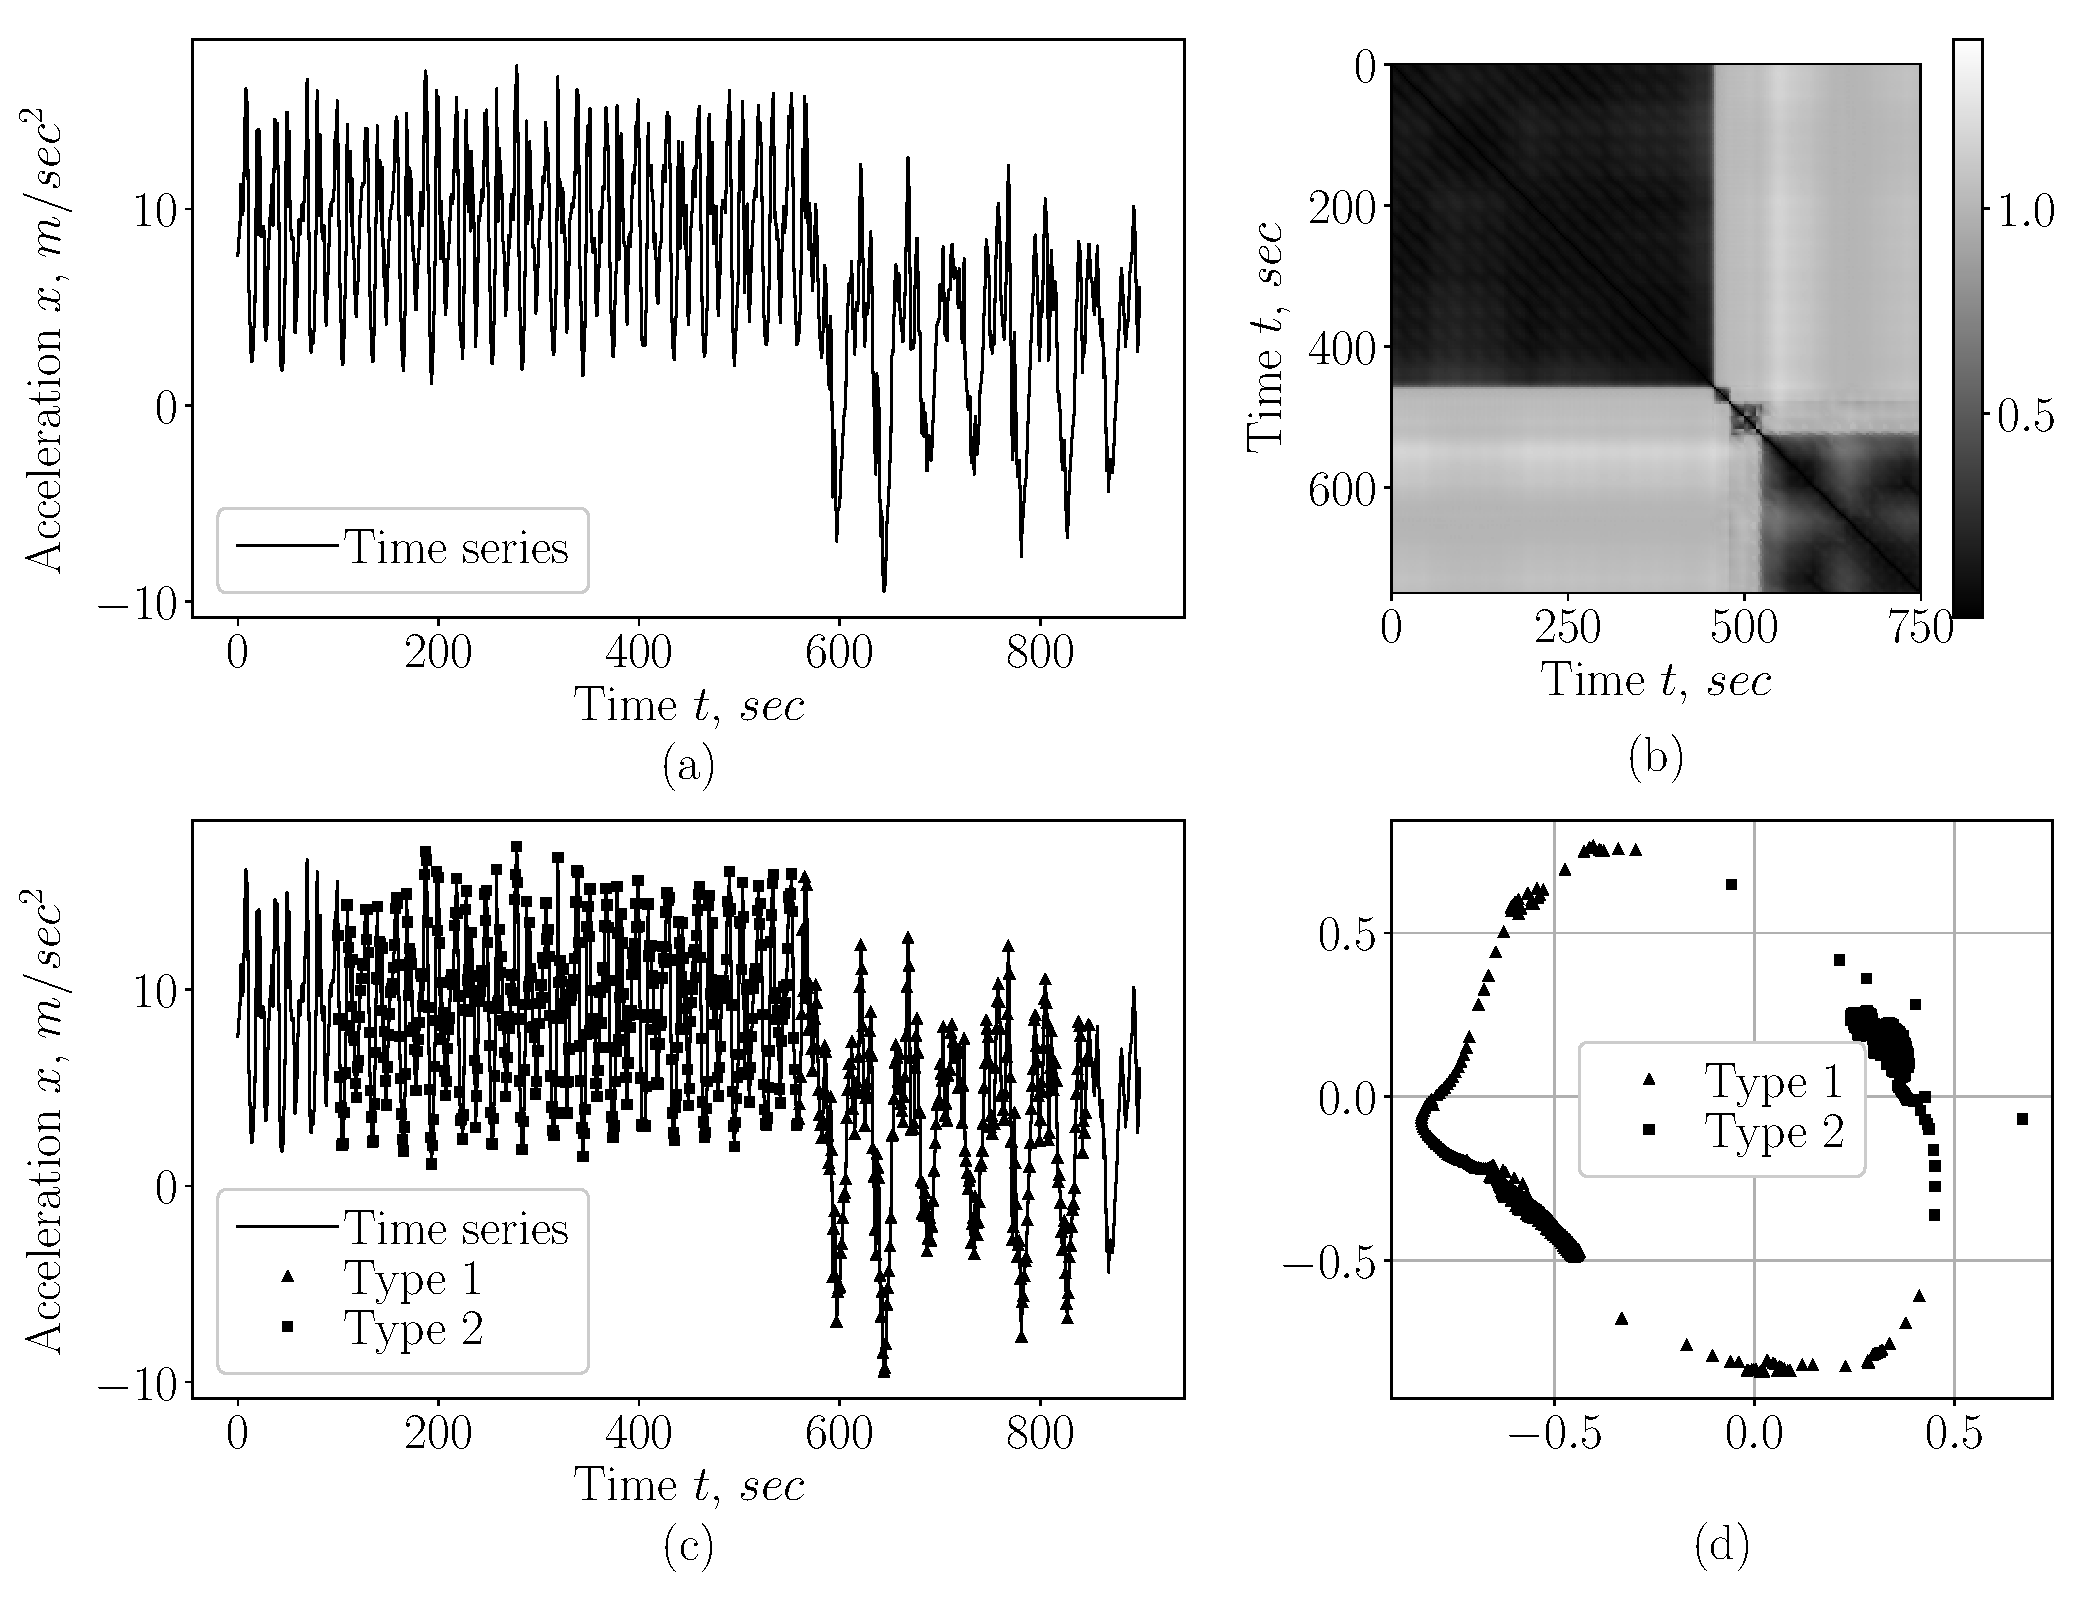
\includegraphics[width=1\textwidth]{results_eng/experiment_clustering}
\caption{The result of the clustering algorithm for the time series "Physical~Motion~2": 
a) a time series; b) the pairwise distance matrix for the time series; c) an example of clustering; d) Multidimensional Scaling of the points into two dimensional subspace by using pairwise distance matrix}
\label{fig:experiment:1}
\end{figure}

In this experiment, the clustering of points in the time series was carried out using matrices of pairwise distances~$(\ref{eq:cl:9})$. 
The experiment was carried out on real and synthetic data, which are described in Table~\ref{table:experiment:1}. 
"Physical Motion" is a time series obtained by using a mobile accelerometer. 
The synthetic time series were constructed by using the first few terms of the Fourier series with random coefficients from the standard normal distribution.
The generation of synthetic time series consisted of two stages.
At the first stage, the short segments~$\textbf{v}$ were generated to build a set of all segments~$\mathbf{V}$.
The second stage is the following random process:
\begin{equation}
\label{eq:exp:1}
\begin{aligned}
\textbf{x} = [\textbf{v}_{1}, \textbf{v}_{2}, \cdots, \textbf{v}_{M}] + \bm{\varepsilon}, \quad \begin{cases}
    \textbf{v}_{1} \sim \mathcal{U}\left(\mathbf{V}\right),\\
    \textbf{v}_{i} = \textbf{v}_{i - 1}, & \text{with probability}~\frac{3}{4}\\
    \textbf{v}_{i} \sim \mathcal{U}\left(\mathbf{V}\right), & \text{with probability}~\frac{1}{4}
\end{cases},
\end{aligned}
\end{equation}
where~$\mathcal{U}\left(\mathbf{V}\right)$ is a uniform distribution on objects from the set~$\mathbf{V},$ and~$\bm{\varepsilon}$ is gaussian noise.

\subsection{Time series segmentation}
\begin{figure}[h!t]\center
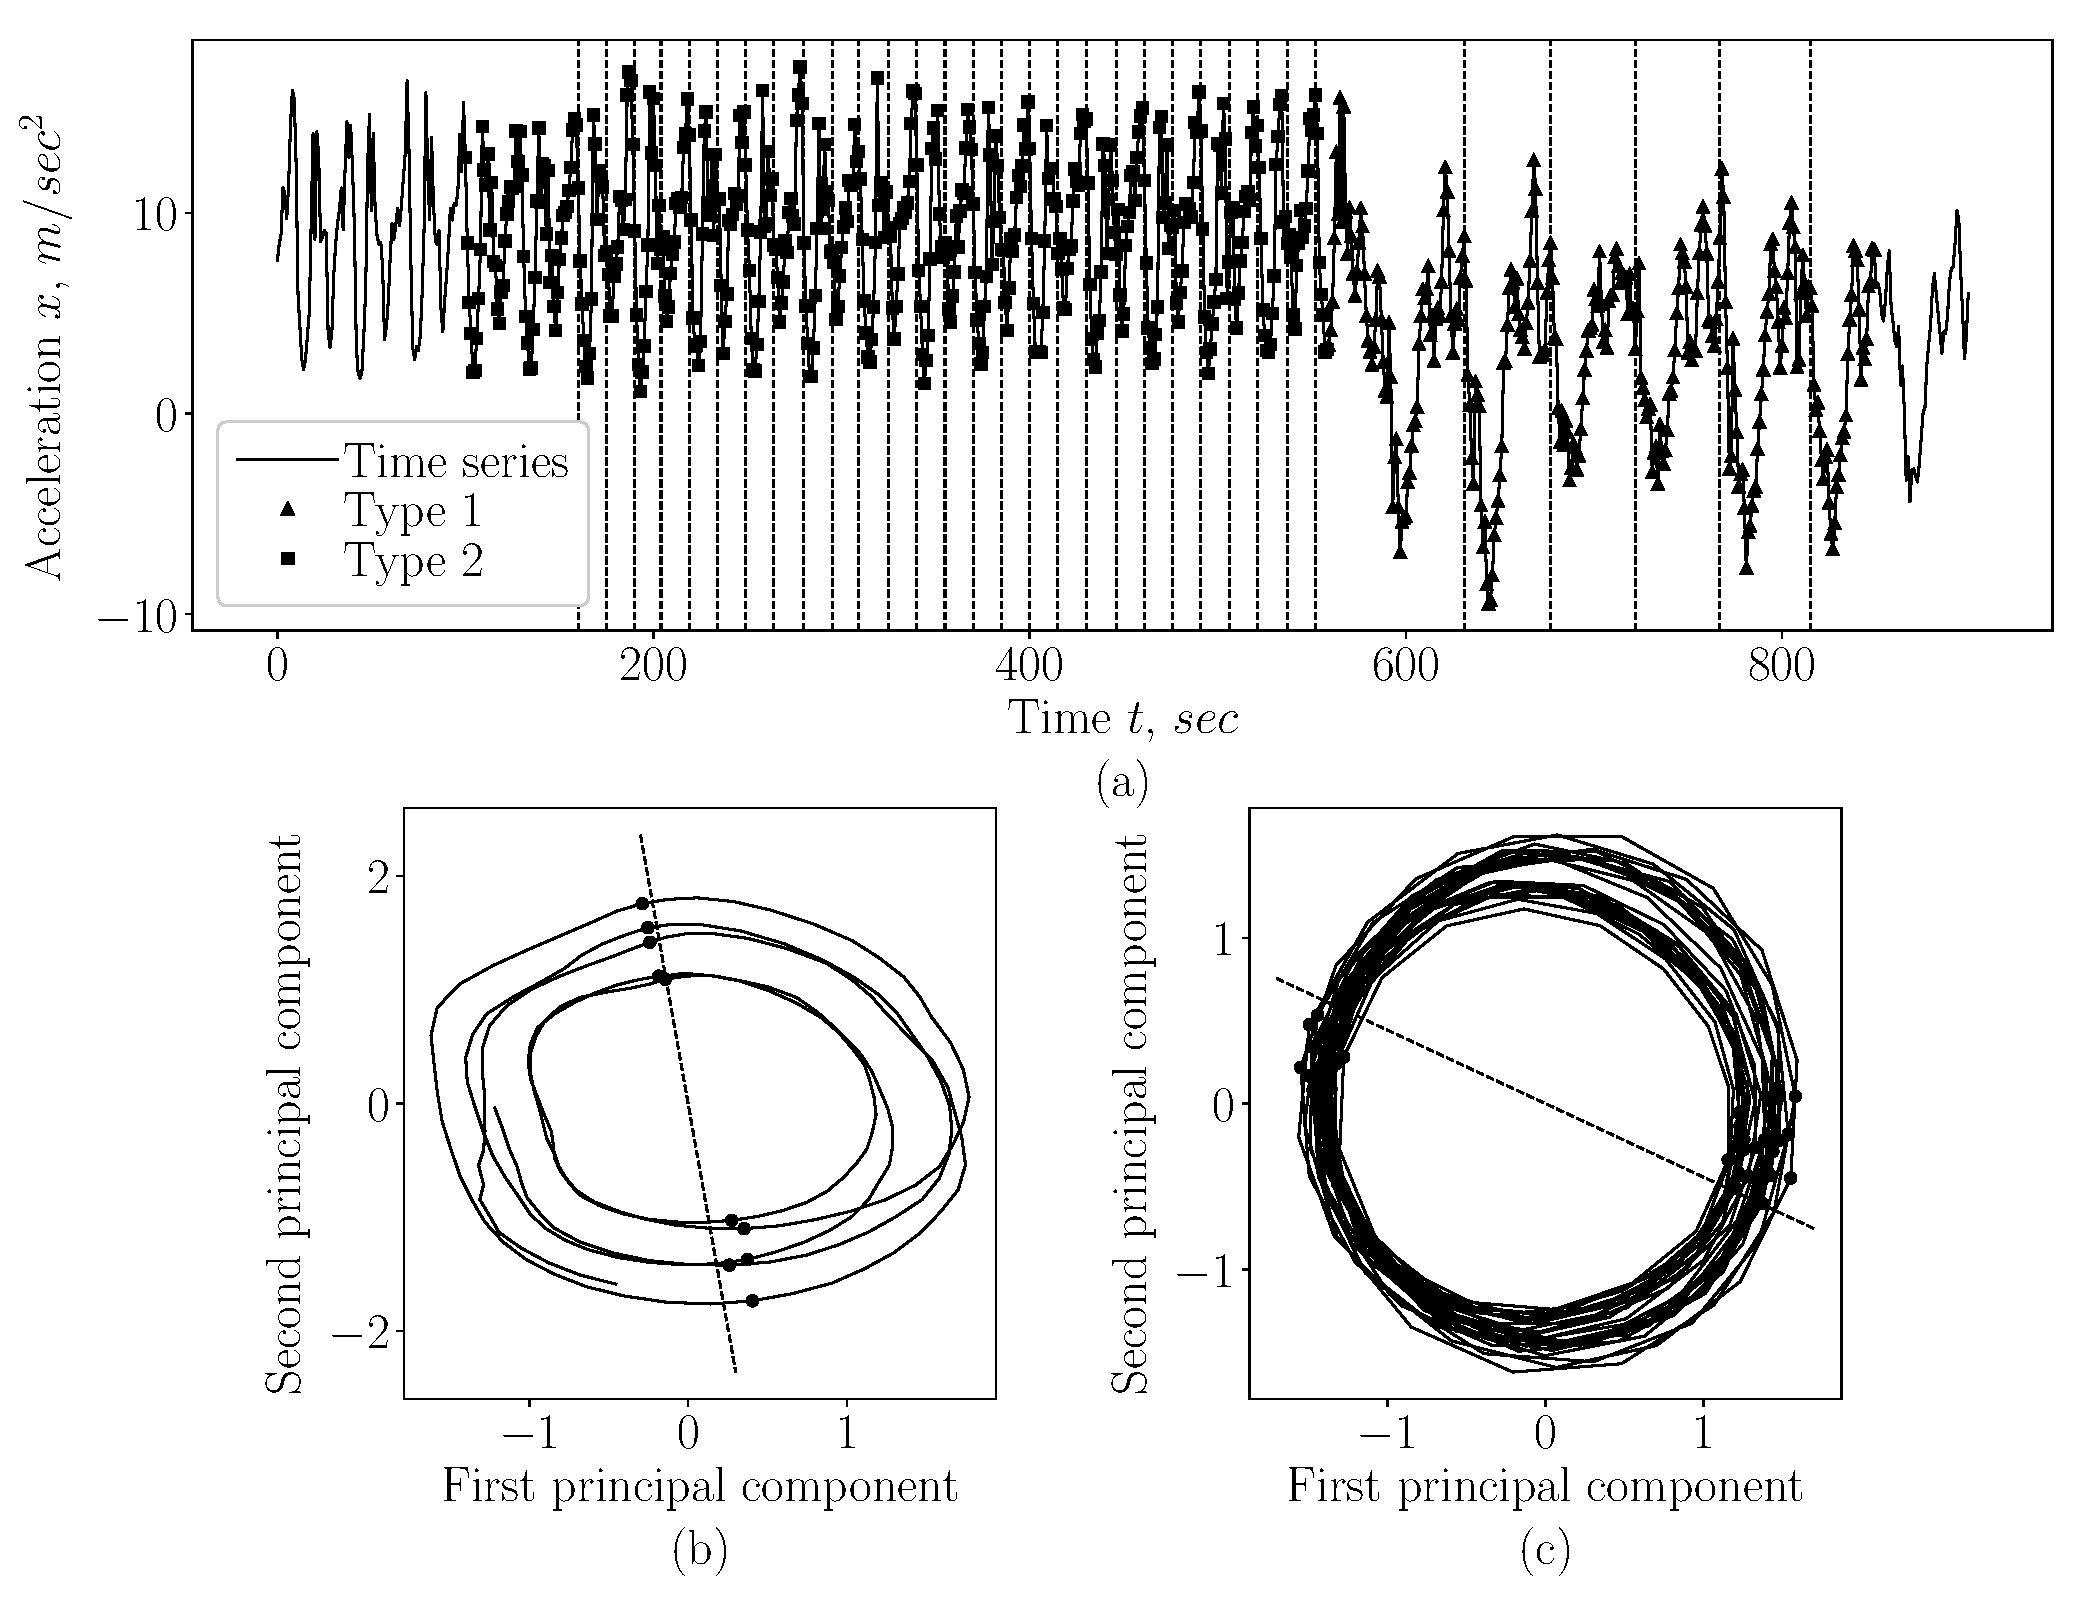
\includegraphics[width=1\textwidth]{results_eng/experiment_segmentation}
\caption{The result of the segmentation algorithm for the time series "Physical~Motion~2": 
a) a time series segmentation; b) a phase trajectory for cluster "Type~1"; c) a phase trajectory for cluster "Type~2"}
\label{fig:experiment:2}
\end{figure}

\begin{table}[h!t]
\begin{center}
\caption{Description of time series in the experiment}
\label{table:experiment:1}
\begin{tabular}{|c|c|c|c|c|}
\hline
	Series,~$\textbf{x}$ &Length,~$N$& Number of segments,~$K$& Period,~$T$ & Error,~$S$\\
	\hline
	\multicolumn{1}{|l|}{Physical~Motion~1}
	& 900& 2& 50& 0.03\\
	\hline
	\multicolumn{1}{|l|}{Physical~Motion~2}
	& 900& 2& 35& 0.08\\
	\hline
	\multicolumn{1}{|l|}{Physical~Motion~3}
	& 900& 2& 30& 0.09\\
	\hline
	\multicolumn{1}{|l|}{Physical~Motion~4}
	& 800& 2& 50& 0.01\\
	\hline
	\multicolumn{1}{|l|}{Synthetic~1}
	& 2000& 3& 40& 0.008\\
	\hline
	\multicolumn{1}{|l|}{Synthetic~2}
	& 2000& 2& 40& 0.06\\
	\hline
	\multicolumn{1}{|l|}{Synthetic~3}
	& 2000& 2& 40& 0.03\\
	\hline
	\multicolumn{1}{|l|}{Synthetic~4}
	& 2000& 2& 40& 0.03\\
	\hline
	\multicolumn{1}{|l|}{Synthetic~5}
	& 2000& 2& 40& 0.04\\
	\hline
	\multicolumn{1}{|l|}{Simple}
	& 1000& 2& 135& 0.14\\
\hline

\end{tabular}
\end{center}
\end{table}

The result of the clustering algorithm for the real time series is shown in the fig.~\ref{fig:experiment:1}. The fig~\ref{fig:experiment:1}.b shows the matrix of pairwise distances for points in the timeline. Time series points can be easily visualised on a plane by using the pairwise distance matrix and the Multidimensional Scaling method~\cite{Borg2005}. The visualisation is shown in the fig.~\ref{fig:experiment:1}.d. Fig~\ref{fig:experiment:1}.c shows the result of clustering points. More results of clustering are presented in Table~\ref{table:experiment:1}.

%\paragraph{Synthetic data.}

%The fig.~\ref{fig_synthetic_series} shows an example of synthetic time series.
%The fig.~\ref{fig_synthetic_series_2} shows an example of a time series in which the number of different segments is~$K = 2$, and the maximum length of segments is~$T = 20$.
%The fig.~\ref{fig_synthetic_series_3} shows an example of a time series in which the number of different segments is~$K = 3$, and the maximum length of segments is~$T = 20$.

%The fig.~\ref{fig_synthetic_distance} illustrates the pairwise distance matrix~$\textbf{M}$ between all pairs of points~$t$ in the time series, which are constructed by using equention~(\ref{eq:cl:9}).
%Time series points can be easily visualized on a plane by using a pairwise distance matrix and a Multidimensional Scaling method~\cite{Borg2005}.
%The fig.~\ref{fig_synthetic_2D} shows the visualization of points on the plane and performed their clustering by using the hierarchical clustering method.

%\paragraph{Real data.}

%The fig.~\ref{fig_real_series} shows an example of real time series obtained using a mobile accelerometer.

%The fig.~\ref{fig_real_distance} illustrates the pairwise distance matrix~$\textbf{M}$ between all pairs of points~$t$ in the time series, which are constructed by using equention~(\ref{eq:cl:9}).
%Time series points can be easily visualized on a plane by using a pairwise distance matrix and a Multidimensional Scaling method~\cite{Borg2005}.
%The fig.~\ref{fig_real_2D} shows the visualization of points on the plane and performed their clustering by using the hierarchical clustering method.

The time series segmentation is shown on the example of real data obtained by using a mobile accelerometer. Segmentation is carried out by using the method that is presented in the work~\cite{motrenko2015}. The method is used for each action within the time series separately.
Fig.~\ref{fig:experiment:2} shows the result of the segmentation algorithm for the time series "Physical~Motion~2". The segmentation result for a cluster "Type~1" is much better than for a cluster "Type~2". This result is easily explained by using fig.~\ref{fig:experiment:2}.b and fig.~\ref{fig:experiment:2}.c. Fig.~\ref{fig:experiment:2}.b shows a phase trajectory for the cluster "Type~1". This phase trajectory has no self-intersections in contrast to the phase trajectory shown in the fig.~\ref{fig:experiment:2}.c.
As a result, for time series with a simple phase trajectory, this method performs the time series segmentation well.

%Time series segmentation is carried out on synthetic and real data. 
%A synthetic time series for this experiment were constructed by using the concatenation of two different sinusoidal signals with different amplitude and frequency.
%The experiment was carried out on real and synthetic data, which are described in the table~\ref{table:3}.

%\paragraph{Synthetic data.}
%The fig.~\ref{fig_simple_segmentation} shows the result of the segmentation for the Simple~1 time series.
%The algorithm is well marked the beginning of the segments.

%The fig.~\ref{fig_simple_segmentation} shows the projections of the phase spaces for both clusters onto their first two main components.

%\paragraph{Real data.}
%The fig.~\ref{fig_simple_segmentation} shows the result of the segmentation for the Physical~Motion~2 time series.
%The algorithm is well marked the beginning of the segments for Type~1 and bad for Type~2.
%The fig.~\ref{fig_simple_segmentation} shows the projections of the phase spaces for both clusters onto their first two main components.
%Bad segmentation was obtained due to self-intersection of the phase trajectory.

\section{Conclusion}


The paper investigated the problem of finding periodic structures in time series.
A method based on local reduction of the phase space dimension was proposed.
An algorithm for searching for segments was proposed. 
The algorithm is based on the principal component method for local dimension reduction.
Proposed the the function of the distance between local basis.
The local bases were interpreted as a features description of a point in the time series.

During the experiment on the real and synthetic data set showed that the proposed method for measuring the distance between the basis well separates points that are related to different type of action, which leads to good clustering of time series points.
The results of the experiment are shown in Table~\ref{table:experiment:1}.
The experiment was carried out segmentation of time series by using the method~\cite{motrenko2015} for each cluster separately.

The proposed method has few disadvantages associated with a large number of assumption on a time series.
These restrictions will be relaxed in subsequent papers.
It is also planned to solve the problem of finding the minimum dimension of the phase space for which the phase trajectory will not have self-intersections.

\begin{thebibliography}{99}
	\bibitem{kwapisz2010}
	\textit{J. R. Kwapisz, G. M. Weiss, S. A. Moore} Activity Recognition using Cell Phone Accelerometers~// Proceedings of the Fourth International Workshop on Knowledge Discovery from Sensor Data, 2010. Vol. 12. P. 74--82.
	
	\bibitem{wang2014}
	\textit{W. Wang, H. Liu, L. Yu, F. Sun} Activity Recognition using Cell Phone Accelerometers~// Joint Conference on Neural Networks, 2014. P. 1185--1190.
	
	\bibitem{Ignatov2015}
	\textit{A. D. Ignatov, V. V. Strijov} Human activity recognition using quasiperiodic time series collected from a single tri-axial accelerometer.~// Multimedial Tools and Applications, 2015.
	
	\bibitem{Olivares2012}
	\textit{A. Olivares, J. Ramirez, J. M. Gorris, G. Olivares, M. Damas} Detection of (in)activity periods in human body motion using inertial sensors: A comparative study.~// Sensors, 12(5):5791–5814, 2012.
	
	\bibitem{cinar2018}
	\textit{Y. G. Cinar and H. Mirisaee} Period-aware content attention RNNs for time series forecasting with missing values~// Neurocomputing, 2018. Vol. 312. P. 177--186.
	
	\bibitem{motrenko2015}
	\textit{A. P. Motrenko, V. V. Strijov} Extracting fundamental periods to segment biomedical signals~// Journal of Biomedical and Health Informatics, 2015,~20(6). P.~1466~-~1476.
	
	\bibitem{lukashin2003}
	\textit{Y. P. Lukashin} Adaptive methods for short-term forecasting~// Finansy and Statistik, 2003.
	
	\bibitem{Ivkin2015}
	\textit{M. P. Kuznetsov,  N. P. Ivkin} Time series classification algorithm using combined feature description~// Machine Learning and Data Analysis, 2015,~11(1). P.~1471--1483.
	
	\bibitem{Katrutsa2015}
	\textit{V. V. Strijov, A. M. Katrutsa} Stresstes procedures for features selection algorithms.~// Schemometrics and Intelligent Laboratory System, 2015.
	
	\bibitem{Borg2005}
	\textit{I. Borg, P. J. F. Groenen} Modern Multidimensional Scaling. --- New York: Springer, 2005. 540 p.
	
	\bibitem{Shiglavsi1997}
	\textit{D. L. Danilov, A. A. Zhiglovsky} Main components of time series: method "Gesenitsa".~---~St.~Petersburg University, 1997.
	
	\bibitem{Ignatov2015}
	\textit{A.D. Ignatov, V. V. Strijov} Human activity recognition using quasi-periodic time series collected from a single triaxial accelerometer.~// Multimedia Tools and Applications, 2015, P.~1--14.

	
\end{thebibliography}

\end{document}

